\begin{figure}[H]
	\center
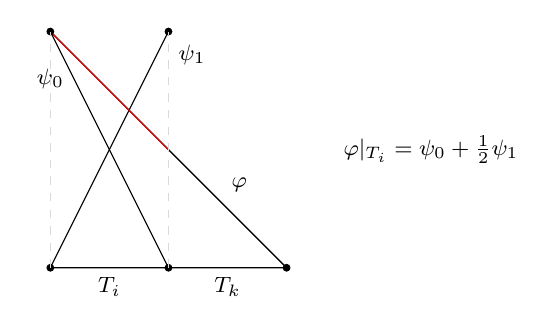
\begin{tikzpicture}[scale=3]
		
		\def \xone{0};
		\def \yone{0};		
		% first rectangle
		\coordinate (A) at (\xone,\yone);
		
        \draw (A) -- ++(1,0) -- ++(-1,1);
        \draw (A) ++(1,0) -- ++(-1,1);
        \draw (A) -- ++(0.5,1);
        \draw (A) ++(0,1) -- ++(0.5,-1);
        \draw[red] (A) ++(0,1) -- ++(0.5,-0.5);
        \filldraw (A)         circle (0.4pt);
        \filldraw (A) ++(1,0) circle (0.4pt);
        \filldraw (A) ++(0,1) circle (0.4pt);
        \filldraw (A) ++(0.5,0) circle (0.4pt);
        \filldraw (A) ++(0.5,1) circle (0.4pt);
        \fill[black,font=\footnotesize] (A) ++(0,0.8)    node {$\psi_0$}
                                        (A) ++(0.6,0.9)  node {$\psi_1$}
                                        (A) ++(0.8,0.35) node {$\varphi$}
                                        (A) ++(1.2,0.5)  node[right] {$\varphi|_{T_i} = \psi_0 + \frac{1}{2}\psi_1$}
                                        (A) ++(0.25,0)   node[below] {$T_i$}
                                        (A) ++(0.75,0)   node[below] {$T_k$};
        \draw[dashed,gray!30!] (A) ++(1/2,0) -- ++(0,1);
        \draw[dashed,gray!30!] (A)			 -- ++(0,1);

        
        
\end{tikzpicture}

\caption{difference of basisfunctions, $T_i \subset T_k$}
\label{ch_mult_other_basis}
\end{figure}